\begin{figure}[H]
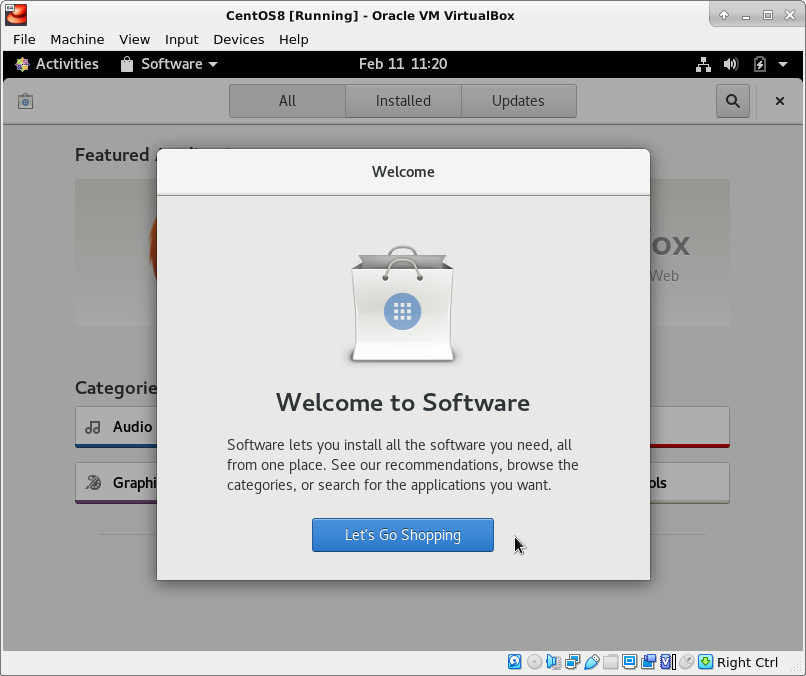
\includegraphics[width=0.9\textwidth]{linuxreader-img019.png}
\end{figure}
{\selectlanguage{dutch}
Rechtsboven kunnen we zoeken op een applicatie, we kunnen echter ook kiezen voor applicaties uit een Categorie. Klikken
we op Graphics \& Photography. Dan vinden we tussen de opties de Gimp. Selecteer de Gimp en klik Install. Er zal
gevraagd worden om het root-wachtwoord, na dit ingevoerd te hebben begint de installatie.}

{\selectlanguage{dutch}
Hierna kan je Software afsluiten of direct de Gimp opstarten.}

\begin{figure}
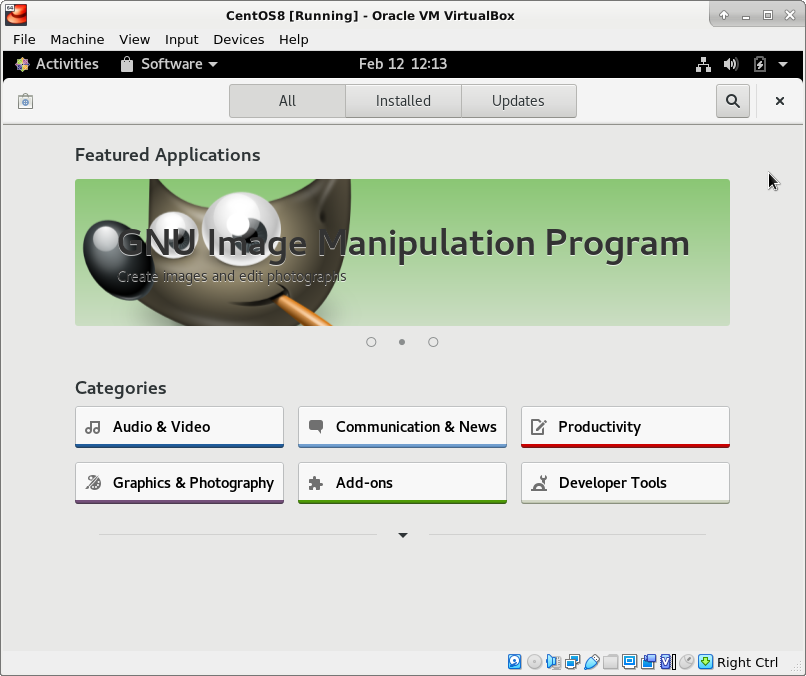
\includegraphics[width=0.9\textwidth]{linuxreader-img020.png}
\end{figure}
